\documentclass[11pt,letterpaper]{article}
\PassOptionsToPackage{hyphens}{url}
\usepackage[margin=.83in,top=.8in,bottom=.8in,headheight=15pt]{geometry}
\usepackage[T1]{fontenc}
\usepackage{lmodern,amsmath,amssymb,mathtools,bm,booktabs,array,graphicx,tikz}
\usetikzlibrary{arrows.meta,positioning,calc,decorations.pathreplacing,patterns}
\definecolor{ink}{HTML}{17344D}\definecolor{accent}{HTML}{087E8B}\definecolor{pale}{HTML}{EDF5F5}\definecolor{gold}{HTML}{AD6B19}
\providecommand{\dd}{\,\mathrm{d}}\providecommand{\R}{\mathbb{R}}
\providecommand{\E}{\mathbb{E}}\providecommand{\Var}{\operatorname{Var}}
\providecommand{\Cov}{\operatorname{Cov}}\providecommand{\diag}{\operatorname{diag}}
\providecommand{\norm}[1]{\left\lVert#1\right\rVert}
\providecommand{\abs}[1]{\left|#1\right|}
\usepackage{microtype,hyperref,fancyhdr,enumitem,amsthm,sectsty,needspace}
\allsectionsfont{\raggedright}
\hypersetup{colorlinks=true,linkcolor=ink,urlcolor=accent,pdfauthor={Zan Ahmad},pdftitle={Membrane voltage and a traveling activation / Lecture notes}}
\setlength{\parindent}{0pt}\setlength{\parskip}{6pt}\linespread{1.07}
\setlist{itemsep=3pt,topsep=4pt,leftmargin=*}
\emergencystretch=2em\clubpenalty=10000\widowpenalty=10000
\pagestyle{fancy}\fancyhf{}\fancyhead[L]{\small Mathematical Cardiology}\fancyhead[R]{\small Lecture 4}
\fancyfoot[L]{\footnotesize Zan Ahmad}\fancyfoot[R]{\footnotesize\thepage}\renewcommand{\headrulewidth}{.3pt}
\newtheorem{proposition}{Proposition}\newtheorem{theorem}{Theorem}\newtheorem{lemma}{Lemma}
\theoremstyle{definition}\newtheorem{definition}{Definition}\newtheorem{example}{Example}
\numberwithin{equation}{section}
\begin{document}
{\small\scshape Mathematical Cardiology\hfill Lecture 4}\par\medskip
{\raggedright\hyphenpenalty=10000\exhyphenpenalty=10000\LARGE\bfseries\color{ink} Membrane voltage and a traveling activation\par}\medskip
{\small Lecture notes}\par\bigskip
A voltage trace, a traveling activation and an electrocardiogram are different mathematical objects. A trace assigns a voltage to each time at one location. A traveling activation also assigns an arrival time to each location. An ECG is a body-surface measurement influenced by distributed electrical sources and the conducting body. We begin with the first two objects and derive exactly what can be inferred from a prescribed traveling waveform.

\section{Charge balance gives a voltage equation}
\hypertarget{note-charge-balance-gives-a-voltage-equation}{}\label{note:charge-balance-gives-a-voltage-equation}
{\small \href{slides.html\#frame=three-different-observations\&step=1}{Slides for this section}}\par
Membrane voltage $V_m$ is the electric potential inside the cell minus that outside. A negative value means lower internal potential under this convention. It is not a negative amount of blood or a count of ions. The membrane separates charge and can be represented, at a selected scale, by capacitance $C_m$. With outward ionic currents taken as positive, charge balance has the form
\begin{equation}
C_m\frac{dV_m}{dt}=I_{\rm applied}-\sum_j I_j.
\end{equation}
The right-hand side is a net current; the left-hand side is the rate of capacitive charge change. Over a short interval, this can instead be read as $C_m\Delta V_m\approx h(I_{\rm applied}-\sum_j I_j)$.

A simple channel-current relation is $I_j=g_j(V_m-E_j)$, where $g_j$ is conductance and $E_j$ is a reversal potential. The direction depends on the difference from $E_j$, not simply on the sign of $V_m$. If conductances are temporarily fixed and applied current is zero, define $g=\sum_jg_j$ and $\overline E=\sum_jg_jE_j/g$, for $g>0$. Then
\[
C_m\frac{dV_m}{dt}=-g(V_m-\overline E).
\]
This resembles the reservoir equation: voltage moves toward a conductance-weighted value with time scale $C_m/g$. An action potential requires the conductances themselves to change; a fixed passive relaxation cannot explain its entire shape.
\section{A gate equation counts opening and closing}
\hypertarget{note-a-gate-equation-counts-opening-and-closing}{}\label{note:a-gate-equation-counts-opening-and-closing}
{\small \href{slides.html\#frame=count-gates-available-to-change\&step=1}{Slides for this section}}\par
Let $n$ be the fraction of gates open. During a small interval $h$, suppose a fraction approximately $\alpha h$ of closed gates open and a fraction approximately $\beta h$ of open gates close. The available closed fraction is $1-n$, so
\[
n_{\rm new}-n\approx h\{\alpha(1-n)-\beta n\}.
\]
The continuous notation is $dn/dt=\alpha(1-n)-\beta n$. At fixed voltage, $\alpha$ and $\beta$ can be treated as fixed positive rates. The equilibrium open fraction is $\alpha/(\alpha+\beta)$, obtained by setting opening and closing rates equal.

If a channel requires four identical independent gates to be open, its open probability is $n^4$, not $4n$. That power uses an independence assumption; merely drawing four gates does not establish it. This is part of the classic Hodgkin--Huxley nerve-model construction, developed for the squid giant axon. Cardiac cells require different current choices and calcium dynamics. These equations explain a modeling structure; the companion does not implement them or relabel a neuronal model as human ventricular tissue.
\section{Specify the waveform that is actually displayed}
\hypertarget{note-specify-the-waveform-that-is-actually-displayed}{}\label{note:specify-the-waveform-that-is-actually-displayed}
{\small \href{slides.html\#frame=the-supplied-waveform\&step=1}{Slides for this section}}\par
The companion uses a prescribed function $F(a)$ of local time since activation, $a$. It joins the following points by straight segments:
\[
\begin{array}{c|rrrrr}
a\ (\mathrm{ms})&0&2&12&160&220\\\hline
F(a)\ (\mathrm{mV})&-85&30&15&0&-85
\end{array}
\]
Before onset and after the event, $F=-85$ mV. The plateau-like part is chosen to make a ventricular-shaped event visible. It is not an ionic calculation or a universal cardiac waveform.

Between two listed ages $a_i<a_{i+1}$, the rule is
\begin{equation}
F(a)=F(a_i)+\frac{a-a_i}{a_{i+1}-a_i}\{F(a_{i+1})-F(a_i)\}.
\end{equation}
The interpolation fraction is dimensionless. This formula reproduces both endpoints and supplies a declared straight-line assumption between them. Changing the function is changing the prescribed waveform, not testing an ion-channel intervention.
\section{Distance becomes delay}
\hypertarget{note-distance-becomes-delay}{}\label{note:distance-becomes-delay}
{\small \href{slides.html\#frame=a-travel-time\&step=1}{Slides for this section}}\par
Let $x\ge0$ be distance in millimeters from the initiating edge and let $c>0$ be a constant speed in mm/ms. Traveling a distance $x$ at that speed takes time $t_a(x)=x/c$. At observation time $t$, the local age is therefore $a=t-x/c$, and
\begin{equation}
V_m(x,t)=F(t-x/c).
\end{equation}
At $x=20$ mm and $c=0.4$ mm/ms, arrival is $50$ ms. At $t=80$ ms the local trace is $30$ ms old. The point at $x=40$ mm has arrival time $100$ ms and has not yet activated at $80$ ms. The formula delays the waveform without changing its amplitude or duration.

A fixed local age $a_0$ satisfies $t-x/c=a_0$, or $x=c(t-a_0)$. Thus every chosen phase of the waveform follows a straight line in a distance-versus-time plot with slope $c$. Halving $c$ doubles every positive arrival time. The unit conversion $0.4$ mm/ms $=0.4$ m/s works because numerator and denominator are both divided by $1000$.
\begin{center}\begin{minipage}{.98\linewidth}\centering
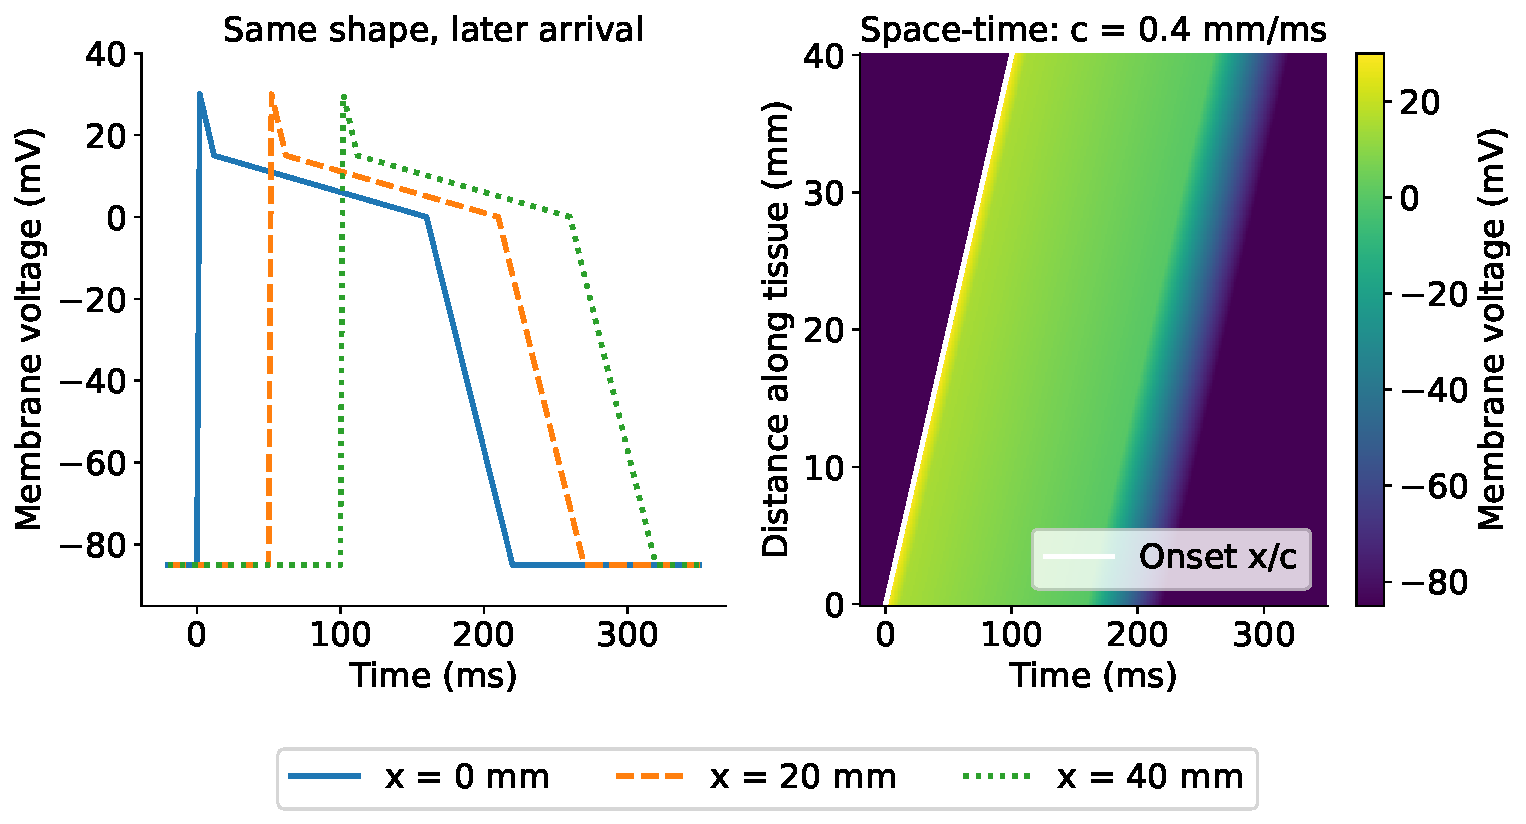
\includegraphics[width=.96\linewidth,height=.57\textheight,keepaspectratio]{trace-and-travel.pdf}\par\smallskip
{\small Original prescribed piecewise-linear voltage shape delayed by x/c with c =\allowbreak{} 0.4 mm/ms. No ion currents are solved.}
\end{minipage}\end{center}
\section{A three-dimensional picture of a one-dimensional rule}
\hypertarget{note-a-three-dimensional-picture-of-a-one-dimensional-rule}{}\label{note:a-three-dimensional-picture-of-a-one-dimensional-rule}
{\small \href{slides.html\#frame=the-slab-inherits-an-imposed-symmetry-panel-1\&step=1}{Slides for this section}}\par
The slab is $40\times30\times8$ mm. The displayed rule has no dependence on width or thickness: $V_m(x,y,z,t)=F(t-x/c)$. At $t=80$ ms, onset has reached $ct=32$ mm for $c=0.4$ and $16$ mm for $c=0.2$. These planes follow from the imposed symmetry. They are not predictions of anisotropic tissue, fiber direction or an anatomical conduction network.

In the normal heart, sinoatrial initiation, atrial activation, atrioventricular delay and specialized ventricular pathways coordinate electrical activity. Excitability and recovery can determine whether a second stimulus propagates. The one-pass translated waveform has no gate recovery or stimulus-response mechanism, so it cannot predict refractory block, reentry or a drug response.

The same limitation can be stated mathematically. Arrival times are inputs determined by $x/c$; no equation here calculates $c$ from channel conductance or coupling. Checking $t_a(2x)=2t_a(x)$ verifies the implementation of the imposed travel law. Testing that law biologically requires recordings at several locations, and testing an ionic explanation requires measurements that distinguish the competing current mechanisms.
\begin{center}\begin{minipage}{.98\linewidth}\centering
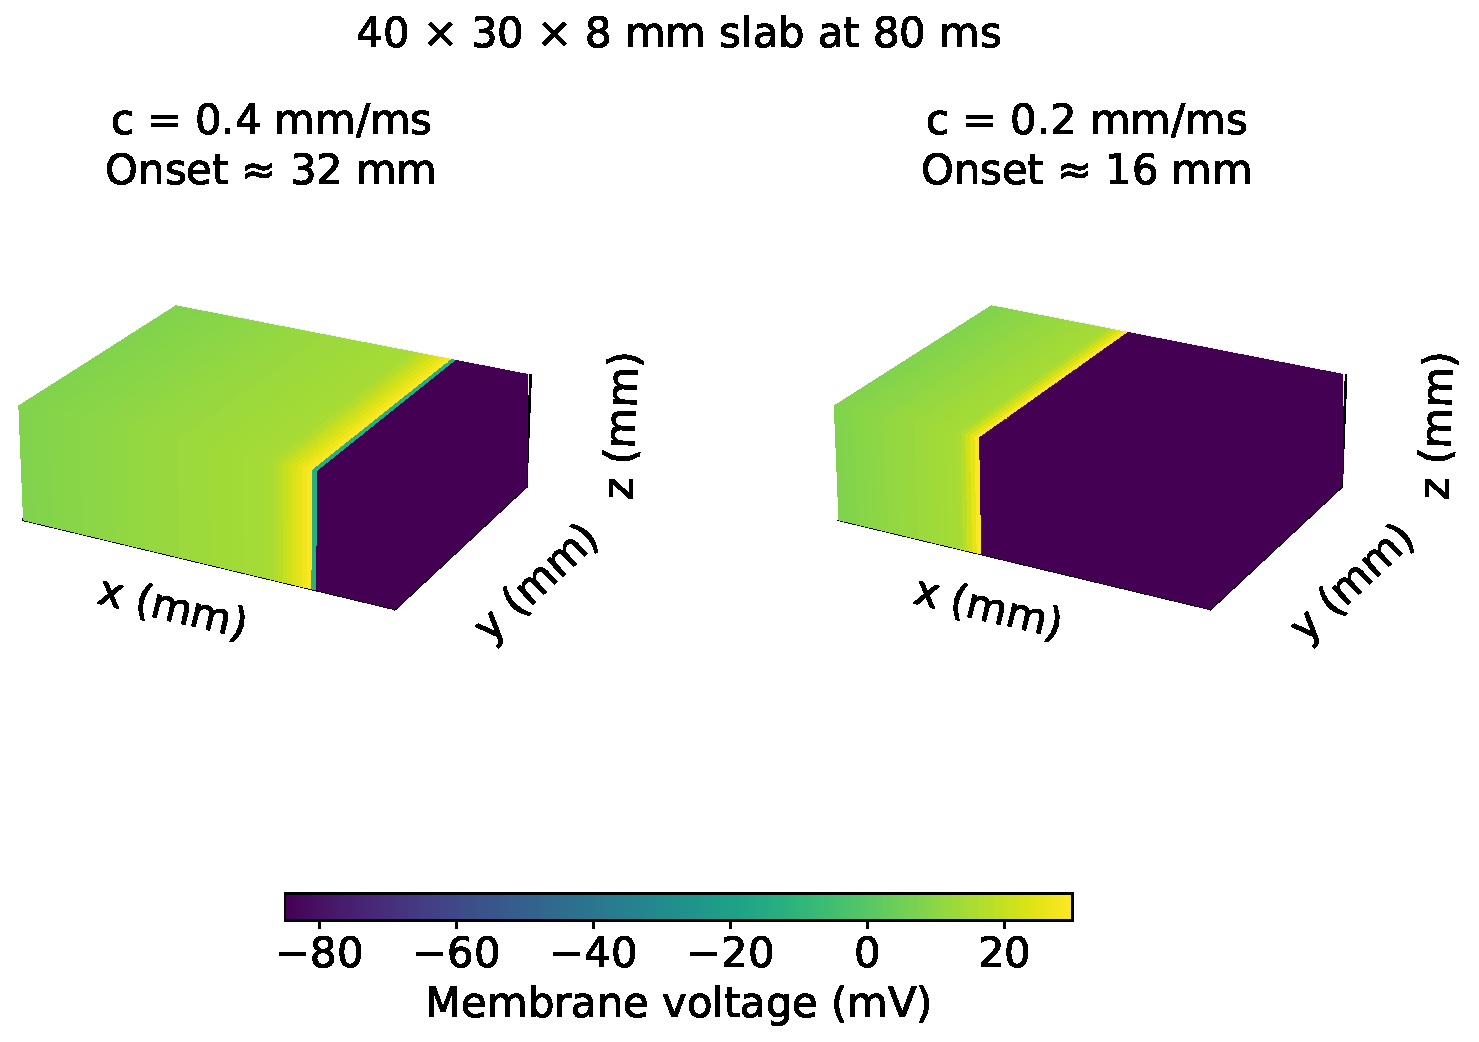
\includegraphics[width=.96\linewidth,height=.57\textheight,keepaspectratio]{activation-slab.pdf}\par\smallskip
{\small Original 40 $\times$ 30 $\times$ 8 mm slab at 80 ms. Speeds 0.4 and 0.2 mm/ms place onset at 32 and 16 mm. This is a geometric display of a prescribed 1D rule, not a 3D tissue solver.}
\end{minipage}\end{center}
\bigskip
\section*{Exercises}
\par\noindent\begin{minipage}{\linewidth}
\subsection*{MC04-E1. Compute delays with units}
Use a homogeneous path with prescribed speed 0.3 mm/ms and positions 15 and 30 mm.

\textbf{a} Find both arrival times.

\end{minipage}\par\medskip
\textbf{b} At absolute time 120 ms, find the local age at each position.

\textbf{c} If speed becomes 0.15 mm/ms, recompute the arrivals and identify which position has activated by 120 ms.

\par\noindent\begin{minipage}{\linewidth}
\subsection*{MC04-E2. Read a local trace and a spatial map}
A drawing shows the same local voltage shape at many locations, each shifted by x/c.

\textbf{a} State the units on a local trace's two axes and on the color scale of a voltage map.

\end{minipage}\par\medskip
\textbf{b} Explain why a later trace need not have smaller amplitude in this construction.

\textbf{c} Give two reasons that the colored slab is not an ECG or a full 3D electrophysiology simulation.

\par\noindent\begin{minipage}{\linewidth}
\subsection*{MC04-E3. Choose a credible extension}
A team proposes to use the supplied one-pass wave to study whether an early second stimulus fails to propagate.

\textbf{a} Name the missing process that makes the proposed claim unsupported.

\end{minipage}\par\medskip
\textbf{b} Name one model addition and one independent observation needed to investigate it.

\textbf{c} Draft a narrower project question that the present rule can answer, with a check and a limitation.

\section*{References}
\noindent\begin{minipage}{\linewidth}
Zan Ahmad, Fall 2023 HEART syllabus. Public PDF pp. 1--2, Course Topics and Course Expectations; editable syllabus pp. 2--3, project requirements.

\end{minipage}\par\medskip
\noindent\begin{minipage}{\linewidth}
Hoppensteadt and Peskin, Modeling and Simulation in Medicine and the Life Sciences, second edition. Printed pp. 124--128; PDF pp. 137--141, section 3.5.

\end{minipage}\par\medskip
\noindent\begin{minipage}{\linewidth}
NHLBI, How the Heart Beats. Electrical conduction sequence.

\url{https://www.nhlbi.nih.gov/health/heart/heart-beats}
\end{minipage}\par\medskip
\noindent\begin{minipage}{\linewidth}
ten Tusscher, Noble, Noble and Panfilov (2004), A model for human ventricular tissue. Abstract; American Journal of Physiology---Heart and Circulatory Physiology 286, H1573--H1589; PMID 14656705.

\url{https://pubmed.ncbi.nlm.nih.gov/14656705/}
\end{minipage}\par\medskip
\end{document}
